\documentclass[12pt]{article}

\usepackage{fontawesome}
\usepackage{hyperref}
\usepackage{xurl}
\usepackage{graphicx}



\hypersetup{
    colorlinks=false,
    pdfborder={0 0 0},
}


\title{SQL Challenges}
\author{
        Adrianna Holden-Gouveia \\
        Website: \url{https://aholdengouveia.name}\\ 
        \date{\vspace{-5ex}}
        %Email: \href{mailto:admin@aholdengouveia.name}{admin@aholdengouveia.name} \\
        \faLinkedin{: aholdengouveia} \\
        \faGithub {: aholdengouveia} \\
        \faTwitter {: aholdengouveia} \\
        }

%S\date{\today}


\begin{document}    

\maketitle

%\begin{abstract}
%This is a template for Linux Administration Lab work
%\end{abstract}
%\tableofcontents

\section*{Objectives:}
\begin{itemize}
    \item The objective of this lab is to work on challenges for SQL problem solving. Prior knowledge SQL is assumed. Students will attempt more real world applications of SQL on interactive methods utilizing a free online tutorial and other resources.
\end{itemize}
\section*{Instructions}

References, a video, a PowerPoint and some notes are available at my website
\url {https://www.aholdengouveia.name/IntroData/sql3.html}

The challenges are here: \url{https://www.hackerrank.com/domains/sql} 
You must do at least X beginner and X intermediate or advanced challenges

\subsection*{Please include answers to the following questions}
    \begin{enumerate}
        \item For each challenge explain the query you used to solve the problem.
        \item What resources did you need for these challenges?
        \item Would you recommend these challenges to others? 
        \item Take screenshots of the solution to each challenge. Make sure to have a note with your name and the term in the screenshot, screenshot should be focused on the note and answer, not the full desktop.  Any screenshots that don't include the note, or are full desktop, or taken with a camera instead of a screenshot won't count and will earn no points. This is an example of what it should look like:        
 
        \begin{figure}[h!]
            \centerline{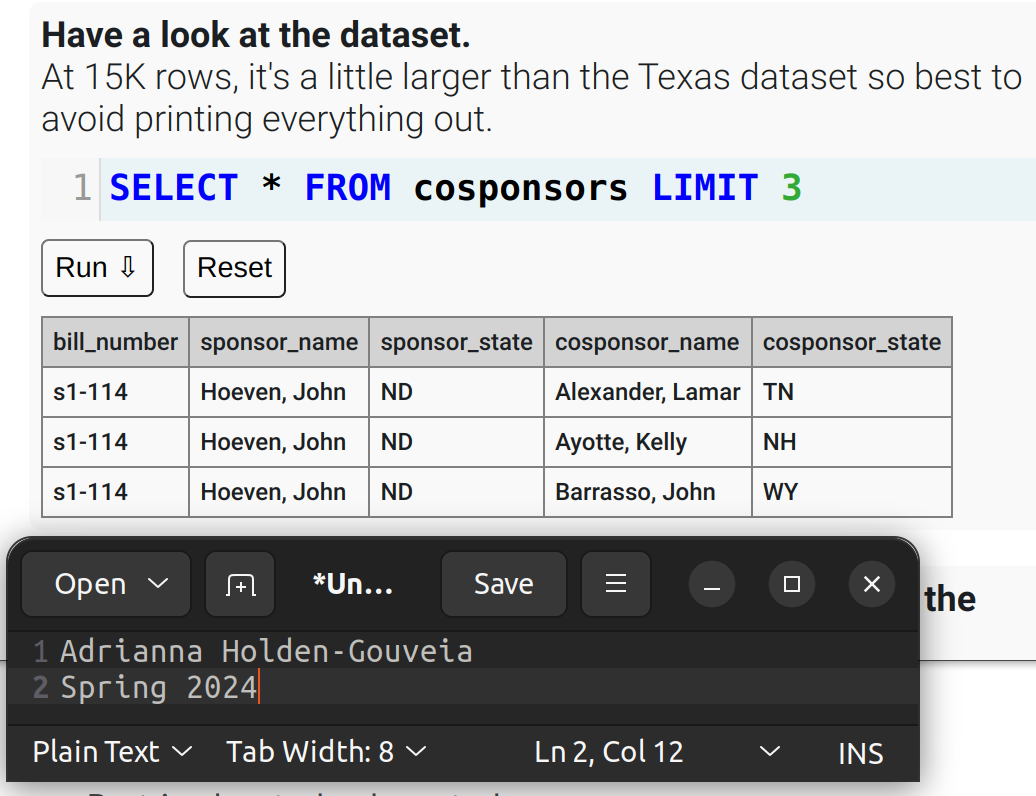
\includegraphics[scale=.2]{Examplewk6.png}}
            \caption{This is an image of what each of your screenshots should look like}

            \end{figure} 
    \end{enumerate}

    \section*{Case Study Recommendation}
You should find a Case Study website that you would recommend to another person.  In your recommendation you should explain why you picked the one you did. You may not include any of the links I've shared in your list, they must be new to you materials and tutorials/videos. 


\section*{Deliverables}
\begin{itemize}
    \item A document containing all requested screenshots
    \item Answers to the above questions
    \item Your case study recommendation.  Review should be at least a paragraph but no more then two pages. 
\end{itemize} 
\end{document}